%%
%% Automatically generated file from DocOnce source
%% (https://github.com/hplgit/doconce/)
%%
%%


%-------------------- begin preamble ----------------------

\documentclass[%
oneside,                 % oneside: electronic viewing, twoside: printing
final,                   % draft: marks overfull hboxes, figures with paths
10pt]{article}

\listfiles               %  print all files needed to compile this document
\usepackage{mathtools}
\usepackage{relsize,makeidx,color,setspace,amsmath,amsfonts,amssymb}
\usepackage[table]{xcolor}
\usepackage{bm,ltablex,microtype}
\usepackage{float}
\usepackage[pdftex]{graphicx}
\usepackage{epstopdf}
\usepackage{verbatim}

\usepackage{fancyvrb} % packages needed for verbatim environments

\usepackage[T1]{fontenc}
%\usepackage[latin1]{inputenc}
\usepackage{ucs}
\usepackage[utf8x]{inputenc}
\usepackage[english]{babel}
\usepackage{lmodern}         % Latin Modern fonts derived from Computer Modern

% Hyperlinks in PDF:
\definecolor{linkcolor}{rgb}{0,0,0.4}
\usepackage{hyperref}
\hypersetup{
    breaklinks=true,
    colorlinks=true,
    linkcolor=linkcolor,
    urlcolor=linkcolor,
    citecolor=black,
    filecolor=black,
    %filecolor=blue,
    pdfmenubar=true,
    pdftoolbar=true,
    bookmarksdepth=3   % Uncomment (and tweak) for PDF bookmarks with more levels than the TOC
    }
%\hyperbaseurl{}   % hyperlinks are relative to this root

\setcounter{tocdepth}{2}  % levels in table of contents



% prevent orhpans and widows
\clubpenalty = 10000
\widowpenalty = 10000

% --- end of standard preamble for documents ---


% insert custom LaTeX commands...

\raggedbottom
\makeindex
\usepackage[totoc]{idxlayout}   % for index in the toc
\usepackage[nottoc]{tocbibind}  % for references/bibliography in the toc

%-------------------- end preamble ----------------------

\begin{document}

% matching end for #ifdef PREAMBLE

\newcommand{\exercisesection}[1]{\subsection*{#1}}


% ------------------- main content ----------------------



% ----------------- title -------------------------

\thispagestyle{empty}

\begin{center}
{\LARGE\bf
\begin{spacing}{1.25}
PHYS 905 - Project 3
\end{spacing}
}
\end{center}

% ----------------- author(s) -------------------------

\begin{center}
{\bf Terri Poxon-Pearson}
\end{center}

    
% ----------------- end author(s) -------------------------

% --- begin date ---
\begin{center}
April 30, 2017
\end{center}
% --- end date ---

\vspace{1cm}

PUT ABSTRACT HERE

\tableofcontents
 
\section{Introduction}

Certain materials exhibit a behavior where the spins of unpaired electrons in the material align in some region of the material.  This is called a domain and had a "macroscopic" spacial extent on the order of mm \cite{LectureNotes}.  This behavior is called Ferromagnetism and Iron, Nickel, and Cobalt are the most common elements which display this behavior.  When an external magnetic field is applied, the domains which are already in aligned with the field grow, taking over the misaligned domains.  Ferromagnetic materials can remain magnetized, even after that external field is removed.

At the same time, these alignments are fighting against thermal excitations which tend to randomize any ordering at the atomic level.  However, at the Curie temperature, magnetic materials undergo a sharp change in their magnetic properties.  This is the temperature at which random thermal nudges overcome the domain's order and spins are forced out of alignment \cite{Curie}.  This temperature can vary from well below room temperature for rare earth metals like Dysprosium, all the way to almost 1400 K for Cobalt.

In this project we are going to study one of the simplest and most common models for ferromagnetic materials, the Ising model.  This model, although very basic, has proven very useful in understanding, not only ferromagnetic materials, but also antiferromagnetic materials, where neighboring spins anti align with one another, leading to no overall magnetization.  The Ising model has even been applied outside of the physical sciences to model a wide variety of situations.  Some of these include modeling people's opinions about the future of the economy, urban segregation, and how languages change over time \cite{otherising}.  We will us the Ising model in two dimensions to explore properties of a materials phase transition from a magnetic to a nonmagnetic material.  We will employ a Monte Carlo method in this study and, eventually, extract the Curie temperature which can be compared to exact results.

This report will begin with an introduction to the Ising model, beginning with the simple case of a 2 by 2 lattice.  We will explain the model and use it to derive important quantities relevant for statistical mechanics.  Then we will implement this system using Monte Carlo methods.  We will then expand the lattice to a larger size and explore aspects of the Monte Carlo simulation, as well as the phase transition.  Finally, we will extract the critical, Curie temperature from our study and compare it with exact results.

\section{Methods}

\subsection{Introduction to the Ising Model}

The Ising model in two dimensions has a simple expression for the energy between two neighboring spins which can be expressed as

\begin{equation*}
E=-J \sum_{\langle k l \rangle}^N s_k s_l.
\end{equation*}

In this expression, $N$ is the total number of spins, $s_k = \pm$ corresponding to electrons that are spin up or spin down, and the symbol $ \langle kl \rangle$ implies that the sum only runs over nearest neighbors.  This sum does not include spins which are diagonal from one another.  In this framework, J is taken to be a positive value and it is taken as the coupling constant expressing the strength of the spin interaction.

In this work, we will not apply an an external field to the system, although that is a simple extension of the energy expression which gives us

\begin{equation*}
E=-J \sum_{\langle k l \rangle}^N s_k s_l - \mathcal{B} \sum_k^N s_k
\end{equation*}

where $\mathcal{B}$ is the strength of the external magnetic field.  Now we can use this energy to develop expressions for relevant quantities from statistical mechanics.

\subsection{The Ising Model on a 2 by 2 Lattice}

We will begin this development by studying the case of a 2 by 2 lattice (4 spins) where each spin can be either up for down.  If we enumerate all possible configurations, there are 16, pictured below.

\begin{equation*}
\begin{split}
&\begin{smallmatrix} -&-\\ -&- \end{smallmatrix}
\qquad
\begin{smallmatrix} +&-\\ -&- \end{smallmatrix}
\qquad
\begin{smallmatrix} -&-\\ -&+ \end{smallmatrix}
\qquad
\begin{smallmatrix} +&+\\ -&- \end{smallmatrix}
\qquad
\begin{smallmatrix} +&-\\ +&- \end{smallmatrix}
\qquad
\begin{smallmatrix} +&-\\ -&+ \end{smallmatrix}
\qquad
\begin{smallmatrix} +&+\\ +&- \end{smallmatrix}
\qquad
\begin{smallmatrix} +&-\\ +&+ \end{smallmatrix} \\ 
\\
\\
&\begin{smallmatrix} +&+\\ +&+ \end{smallmatrix}
\qquad
\begin{smallmatrix} -&+\\ -&- \end{smallmatrix}
\qquad
\begin{smallmatrix} -&-\\ +&- \end{smallmatrix}
\qquad
\begin{smallmatrix} -&-\\ +&+ \end{smallmatrix}
\qquad
\begin{smallmatrix} -&+\\ -&+ \end{smallmatrix}
\qquad
\begin{smallmatrix} -&+\\+-&- \end{smallmatrix}
\qquad
\begin{smallmatrix} +&+\\ -&+ \end{smallmatrix}
\qquad
\begin{smallmatrix} -&+\\ +&+\end{smallmatrix} 
\end{split}
\end{equation*}

We can enumerate the energy and the magnetization for each of these configurations where the energy is defined above and the magnetization is defined as 

\begin{equation*}
\mathcal{M}_i = \sum_{j=1}^N s_j
\end{equation*}

where the sum runs over all spins for a given configuration $i$.  These quantites are in the table below.

\begin{center} 
\begin{tabular}{ |c|c|c|c| }
\hline
Number of Spin Ups & Number of Configurations & Energy & Magnetization \\
\hline
0 & 1 & -8J  & -4\\ 
1& 4  & 0  & -2\\ 
2 & 4 & 0  & 0\\ 
2 & 2 & 8J & 0 \\
3 & 4 & 0  & 2\\ 
4 & 1 & -8J  & 4\\ 
\hline
\end{tabular}
\label{table:test}
\end{center}

Note that there are two kinds of configurations with 2 spin ups.  This configuration results in 0 energy if the spin up points are adjacent to one another, but has a positive energy if they are diagonal from one another.

Now we have the energies, we can compute the partition function, which is defined as

\begin{equation*}
Z=\sum_{i=1}^M e^{-\beta E_i}
\end{equation*}

where the sum is over all microstates $M$ and $\beta = 1/(kT)$. In the case of the two dimensional lattice, Z is equal to

\begin{equation*}
\begin{split}
Z & =2e^{-8J \beta} +e^{8J \beta} + e^{8J \beta} + 12 e^{0}\\
& = 2e^{-8J \beta} +2e^{8J \beta}+12\\
& = 4 (3+cosh(8 J \beta)).
\end{split}
\end{equation*}

We can define a probability distribution using the partition function

\begin{equation*}
P_i(\beta)= \frac{e^{i \beta E_i}}{Z}
\end{equation*}

And the mean value of some quantity of interest is 

\begin{equation*}
\langle X \rangle = \sum_{i=1}^M X_i P_i.
\end{equation*}

Using this, the expectation value of the energy is 

\begin{equation*}
\begin{split}
\langle E \rangle & = \frac{-8J e^{8 J \beta}+8J e^{-8 J \beta} -8J e^{8 J \beta} + 8J e^{-8 J \beta}}{12+2e^{-8 J \beta} + 2e^{8 J \beta}} \\
& = \frac{-8 J sinh(8 \beta J)}{3 + cosh(8 \beta J)}.
\end{split}
\end{equation*}

The mean magnetization is

\begin{equation*}
\begin{split}
\langle |M| \rangle & = \frac{4 e^{8 J \beta}+(4+4)2 e^{0} + 4 e^{8 J \beta} }{12+2e^{-8 J \beta} + 2e^{8 J \beta}} \\
& = \frac{8e^{8 J \beta}+16}{12+2e^{-8 J \beta} + 2e^{8 J \beta}} \\
& = \frac{2(2+e^{8 J \beta})}{3 + cosh(8 \beta J)}.
\end{split}
\end{equation*}

The specific heat can be defined as 

\begin{equation*}
C_V=\frac{1}{T^2} (\langle E^2 \rangle - \langle E \rangle ^2).
\end{equation*}

We can easily find $\langle E^2 \rangle$ in the same way as before, giving us

\begin{equation*}
\begin{split}
\langle E^2 \rangle & = \frac{64J^2 e^{8 J \beta}+64J^2 e^{-8 J \beta} +64J^2 e^{8 J \beta} + 64J^2 e^{-8 J \beta}}{12+2e^{-8 J \beta} + 2e^{8 J \beta}} \\
& = \frac{64 J^2 cosh(8 \beta J)}{3 + cosh(8 \beta J)}.
\end{split}
\end{equation*}

This leaves us with a final expression for the heat capacity

\begin{equation*}
\begin{split}
C_V & =\frac{1}{T^2} \Big( \frac{64 J^2 cosh(8 \beta J)}{3 + cosh(8 \beta J)}-  \Big(\frac{8 J sinh(8 \beta J)}{3 + cosh(8 \beta J)}\Big)^2 \Big) \\
&=\frac{64 J^2}{T^2}  \frac{1+3 cosh(8J \beta)}{(3 + cosh(8J \beta))^2}.
\end{split}
\end{equation*}

There is a very similar expression for the magnetic susceptibility 

\begin{equation*}
\chi=\frac{1}{T} (\langle M^2 \rangle - \langle |M| \rangle ^2).
\end{equation*}

The value of $\langle M^2 \rangle$ is given by

\begin{equation*}
\begin{split}
\langle M^2 \rangle & = \frac{16 e^{8 J \beta}+(4+4)4e^0 +16 e^{8 J \beta}}{12+2e^{-8 J \beta} + 2e^{8 J \beta}} \\
& = \frac{8(e^{8J\beta}+1)}{3 + cosh(8 \beta J)},
\end{split}
\end{equation*}

so the susceptibility can be written as 

\begin{equation*}
\begin{split}
\chi & =\frac{1}{T} \Big( \frac{8(e^{8J\beta}+1)}{3 + cosh(8 \beta J)} -  \Big(\frac{2(2+e^{8 J \beta})}{3 + cosh(8 \beta J)}\Big)^2 \Big) \\
&=\frac{4}{T}  \frac{3+4 cosh(8J \beta) + 2 sinh(8 J \beta)}{(3 + cosh(8J \beta))^2}.
\end{split}
\end{equation*}

\subsection{The Metropolis Algorithm and Detailed Balance}

In order to perform our calculations, we need the partition function that describes the physical situation.  For the case of the 2 by 2 lattice, it is simple to write this function explicitly, but as the size of the grid grows to large values, the partition function becomes intractable to write explicitly.  This is true in almost every physical application. Therefore, we need some methodology which avoids calculating the partition function explicitly.  This is where the Metropolis algorithm and detailed balance come in.

Suppose we have some PDF, $w(t)$ that evolves via a transition probability $W$ such that 

\begin{equation*}
w_i(t=\epsilon)=W(j \rightarrow i) w_j(t=0),
\end{equation*}

then we can write the action of $W$ as 

\begin{equation*}
w_i(t+1) = \sum_j W_{ij}w_j(t).
\end{equation*}

In the case of the Ising model, $w$ depends on the partition function, which we often cannot write explicitly, additionally, we do not have an analytic form for the transition probability, W.  Therefore, we can choose to model the transition probability as the product of two probabilities, one probability for accepting a move from i to j (A) and one that makes the transition to i from j (T).  We can now express the prbability as

\begin{equation*}
W(j \rightarrow i) = T( j \rightarrow i) A(j \rightarrow i).
\end{equation*}

$W$, $w$, $A$, and $T$ are all probabilities and, therefore, must be between 0 and 1 and their sums over all states must be normalized.  Now we can define the probability of being in state $i$ after some time in terms of our newly defined transition probability.

\begin{equation*}
w_i(t+1)=\sum_j \lbrack w_j(t)T_{j \rightarrow i}A_{j \rightarrow i} + w_i(t)T_{i \rightarrow j} (1-A_{i \rightarrow j}) \rbrack
\end{equation*}

Then we can apply the condition that $\sum_j T_{i \rightarrow j}=1$, leaving us with

\begin{equation*}
w_i(t+1)= w_i(t) +\sum_j \lbrack w_j(t)T_{j \rightarrow i}A_{j \rightarrow i} - w_i(t)T_{i \rightarrow j}A_{i \rightarrow j} \rbrack.
\end{equation*}

We can rearrange this expression as

\begin{equation*}
w_i(t+1)- w_i(t) = \sum_j \lbrack w_j(t)T_{j \rightarrow i}A_{j \rightarrow i} - w_i(t)T_{i \rightarrow j}A_{i \rightarrow j} \rbrack.
\end{equation*}

This is very similar to the Master equation given by

\begin{equation*}
\frac{dw_i(t)}{dt}=\sum_j \lbrack W(j \rightarrow i) w_j - W(i \rightarrow j) w_i \rbrack.
\end{equation*}

This equation states that the rate that a system moves from state $j$ to state $i$ is balanced by the rate at which the system transtitions from $j$ to $i$.  In equilibrium, this should be equal to 0.  That allows us to write

\begin{equation*}
\sum_j w_j T_{j \rightarrow i}A_{j \rightarrow i} = \sum_j w_i T_{i \rightarrow j}A_{i \rightarrow j}
\end{equation*}

We recongnize the product of the transition probabilities on the right side as $W_{ij}$ and we know that this probability is normalized when we sum over all final states, j.  This allows us to rewrite the expression as

\begin{equation*}
w_i=\sum_j w_j W_{j \rightarrow i}.
\end{equation*}

This condition, however, is not sufficient to guarantee that we arrive at the correct distribution in the system.  We just apply the additional condition of detailed balance, which can be written

\begin{equation*}
W(j \rightarrow i)w_j = W(i \rightarrow j) w_i
\end{equation*}

such that, at equilibrium, we have

\begin{equation*}
\frac{W(j \rightarrow i)}{W(i \rightarrow j)}=\frac{w_i}{w_j}.
\end{equation*}

Finally, in terms of $A$ and $T$, this gives is

\begin{equation*}
\frac{T_{j \rightarrow i}A_{j \rightarrow i}}{T_{i \rightarrow j}A_{i \rightarrow j}}=\frac{w_i}{w_j}.
\end{equation*}

$w_i$ and $w_j$ both take the form of a Boltzmann distribution, with the partition function, $Z$, in their denominators so this proportion can be calculated, independent of Z. This can be rearranged to read

\begin{equation*}
\frac{A_{j \rightarrow i}}{A_{i \rightarrow j}}=\frac{T_{i \rightarrow j}w_i}{ T_{j \rightarrow i}w_j}.
\end{equation*}

Detailed balance asumes that $T_{i \rightarrow j}=T_{j \rightarrow i}$, causing a cancelation.  If we insert the expression for the Boltzmann distribution for $w$, we now have

\begin{equation*}
\frac{A(j \rightarrow i)}{A(i \rightarrow j)}=e^{-\beta (E_i-E_j)}.
\end{equation*}

If we think about an application to a system with many different energy states, we know that the physical system will tend towards the lowest energy state, but our system must also be ergodic, meaning that it must be possible for the system to reach any possible state from any starting position.  This means that our algorithm must encode transitions to lower energies after many transitions, but also allow for many paths which include midpoints that reach higher energy states.  One way to encode this is

\begin{equation*}
A(j \rightarrow i) = \begin{cases}
e^{-\beta(E_i-E_j)} & \text{if} \ E_i-E_j > 0 \\
1 & \text{else}
\end{cases}
\end{equation*}

where a transition to a lower energy state is always accepted, but a transition to a higher energy state is accepted with some probability depending on the energy difference.  This is the heart of the Metropolis algorithm we will use in our calculation.

\subsection{Phase Transitions in the Ising Model}

Near the critical temperature, many physical properties are modeled using a simple power law.  For example, the magnetization, heat capacity, and susceptibility are modeled as 
\[
  \langle M(T) \rangle \sim \left(T-T_C\right)^{\beta},
\]

\[
  C_V(T) \sim \left|T_C-T\right|^{\alpha},
\]

\[
  \chi(T) \sim \left|T_C-T\right|^{\gamma},
\]

with the critical exponents $\beta=1/8$, $\alpha = 0$, and $\gamma = 7/4$, respectively.

We can also think about the correlation length of a system undergoing phase transition.  When a material is high above the critical temperature, we expect the correlation length to be on the order of lattice spacing.  As the temperature decreases and approaches $T_C$, we expect the correlation length to increase. This behavior can be modeled as 

\[
  \xi(T) \sim \left|T_C-T\right|^{-\nu}.
\]

where $\nu=1$.

A second-order phase transition is characterized by a
correlation length which is on the order of the size of the system.
Since our model is confined to a finite lattice, $\xi$ will
be proportional with the size of the lattice.  it is possible to relate the behavior at finite lattices with the results for an infinitely large lattice.
That relation is

\begin{equation}
 T_C(L)-T_C(L=\infty) = aL^{-1/\nu},
\end{equation}
where $a$ a constant and  $\nu$ was defined above.
At $T=T_C$, we can use this relationship to define the mean magnetization, heat capacity and susceptibility as

\[
  \langle {\cal M}(T) \rangle \sim \left(T-T_C\right)^{\beta}
  \rightarrow L^{-\beta/\nu},
\]

\[
  C_V(T) \sim \left|T_C-T\right|^{-\gamma} \rightarrow L^{\alpha/\nu},
\]

\[
  \chi(T) \sim \left|T_C-T\right|^{-\alpha} \rightarrow L^{\gamma/\nu}.
\]


\section{Code and Implementation}

All of the programs, results, and benchmarks for this work can be found in my GIT repository ( https://github.com/poxonpea/PHYS905 ).  All codes for this project were written in FORTRAN.

\subsection{General Algorithm for Code}

The heart of this process is in the Metropolis algorithm which is shown in Figure \ref{fig:metropolis}

\begin{figure}[H]\label{fig:metropolis}
  \centering
    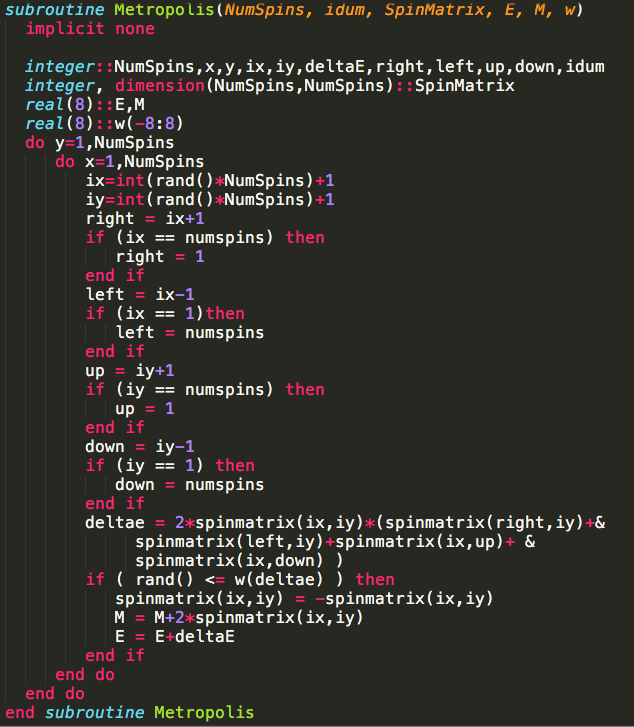
\includegraphics[width=1.0 \textwidth]{Metropolis}
    \caption{The implementation of the Metropolis algorithm used in the Monte Carlo simulation of the Ising Model}
\end{figure}

Below is a general overview of the algorithm for our Monte Carlo code for solving the Ising model

\begin{enumerate}
\item Using a random number generator, choose a random position on the lattice and compute the energy of that state.
\item Flip only one spin in that configuration and compute the new energy of the state.
\item Calculate the energy difference between these two state.
\item If the energy difference is less than 0, we accept the transition.
\item If the energy difference is greater than 0, we calculate $w=e^{-\beta \Delta E}$
\item We generate a random number between 0 and 1.  If that number is less that $w$, we accept the change.  If not, we keep the old configuration.
\item Update expectation values for various quantities.
\item Repeat these steps for each desired Monte Carlo iteration at every desired energy.
\end{enumerate}




\section{Results and Discussion}

\subsection{Comparing Results to Analytic 2 by 2 System}

The first test of our code is to compare our results from our Monte Carlo simulations to the analytic results we achieved for the 2 by 2 case.  All results for our code will be normalized to the size of lattice so that we can compare across calculations.  Therefore, all of the results we obtained before should be divided by four.  In this comparison, we will study the behavior at T=1.0 in units of $kT/J$.  All our or calculations started with a configuration where all spins are aligned, which is the configuration that we expect at low temperature.

The table below gives the results of the calculations, including the relative error when comparing to the analytical values.  For $T=1$, the exact results yield $\langle E \rangle = -1.99598$, $\langle |M| \rangle = 0.998661$ ,$C_V = 0.0320823 $, and $ \chi = 0.00401074$.

\begin{center} 
\begin{tabular}{ |c|c|c|c|c|c|c|c|c| }
\hline
Cycles & $E/N$ & $\epsilon$ & $|M|/N$ & $\epsilon$ &  $C_V/N$ & $\epsilon$ & $\chi/N$ & $\epsilon$ \\
\hline
10 & -1.8182 & 0.0891 & 0.9091 & 0.0869 & 1.3223 & 40.2163 & 0.3306 & 81.4232 \\
50 & -1.9608 & 0.0176 & 0.9894 & 0.0183 & 0.3076 & 8.5870 & 0.0769 & 18.1719 \\
100 & -1.9208 & 0.0377 & 0.9703 &  0.0284 & 0.6086 & 17.9689 & 0.0955 & 22.8063 \\
500 & -1.9521 & 0.0290 & 0.9820 & 0.0166 & 0.3741 & 10.6592 & 0.0586 & 13.6080 \\
1000 & -1.9740 & 0.0110 & 0.9905 & 0.0082 & 0.2051 & 5.3927 & 0.3061 & 6.6317 \\
5000 & -1.9908 & 2.5953E-3 & 0.9966 & 2.0625E-2 & 0.0732 & 1.2831 & 0.0112 & 1.7804 \\
10000 & -1.9928 & 1.5939E-3 & 0.9974 & 1.3123E-3 & 0.0574 & 0.7887 & 8.6711E-3&1.1620 \\
50000 &-1.9945 & 7.5256E-4 & 0.9981& 5.8151E-4& 0.0440 & 0.3726 & 5.9893E-3&0.4923 \\
100000 & -1.9955 & 2.6162E-4 & 0.9985 & 2.0301E-4& 0.0363 & 0.1305 & 4.721E-3&0.17697\\
500000 & -1.9961 & 7.9066E-5 & 0.9987 & 4.9233E-5&0.0308&0.0393&3.8735E-3& 0.0342 \\
1000000&-1.9961 &4.9031E-5 & 0.9987 & 2.4270E-5&0.0313&0.0244&3.9692E-3&0.01036 \\
\hline
\end{tabular}

\label{table:test}
\end{center}

From this table, we can see that we can reach good agreement for the energy and magnetism very quickly, although this is not surprising because we began the simulation in a configuration that is highly favored at low temperature.  It took much longer, however, to reach good agreement with the heat capicity and susceptibility.  In fact, it took about a million Monte Carly cycles to reach agreement on the order of a couple percent.

\subsection{Equilibrium Time}

We can ask ourselves how long it takes for our spin system to settle on its most likely state.  In a sense, the number of Monte Carlo cycles represents the passing of time, so we can examine how many cycles it takes for the calculation to reach equilibrium.  Here we studied this by looking at both the energy and the magnetization as a function of the number of Monte Carlo cycles (time).  We performed this calculation at two different temperature, T=1 and T=2.4.  For both cases we began the calculation from two different orientations: an ordered, spin up configuration, and a random configuration.  Those results are shown below.

\begin{figure}[H]\label{fig:MCEnergy}
  \centering
    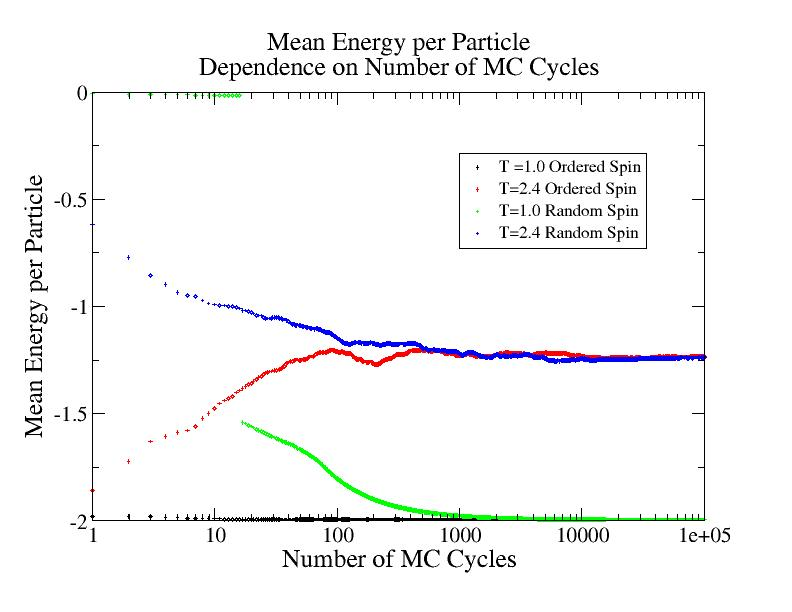
\includegraphics[width=1.1 \textwidth]{MCEnergy.jpg}
    \caption{The mean energy of the 20 by 20 system as a function of the number of Monte Carlo Cycles.  The calculation is repeated at T=1 and T=2.4.  For each case, the calculation is performed with an initial spin configuration that is random and an initial spin configuration that is ordered, with all spins pointing up.}
\end{figure}

For all four cases, the energy levels out, indicating the system seems to come to equilibrium, by about 1,000 Monte Carlo cycles.  Conservatively, waiting until 10,000 cycles eliminates almost all further variation.  It is worth noting that the case of T=1 with an ordered configuration comes to equilibrium much faster, but this is because the beginning configuration is already very close to the equilibrium state.

\begin{figure}[H]\label{fig:MCMag}
  \centering
    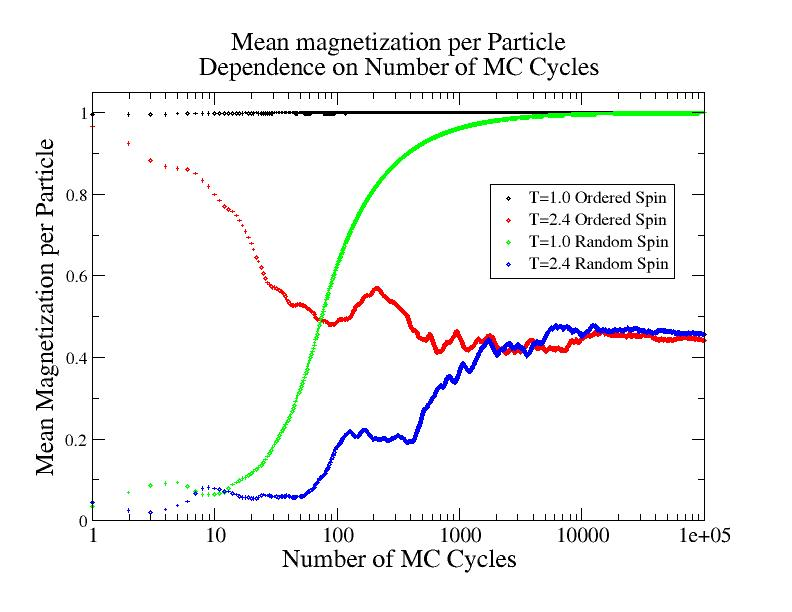
\includegraphics[width=1.1 \textwidth]{MCMag.jpg}
    \caption{The mean magnetization of the 20 by 20 system as a function of the number of Monte Carlo Cycles.  The calculation is repeated at T=1 and T=2.4.  For each case, the calculation is performed with an initial spin configuration that is random and an initial spin configuration that is ordered, with all spins pointing up.}
\end{figure}

For all four cases, the magnetization levels out, indicating the system seems to come to equilibrium, by about 10,000 Monte Carlo cycles.  Again, the case of T=1 with an ordered configuration comes to equilibrium much faster, but this is because the beginning configuration is already very close to the equilibrium state.  This test seems to indicate that about 10,000 cycles are necessary to get reliable values for $\langle E \rangle$ and $\langle |M| \rangle$.

Finally, we can look at the behavior of the number accepted configuration as a function of the time.  The plot below demonstrates this behavior for the 20 by 20 system at three different temperature, T=1,3,and 5.

\begin{figure}[H]\label{fig:acceptplot}
  \centering
    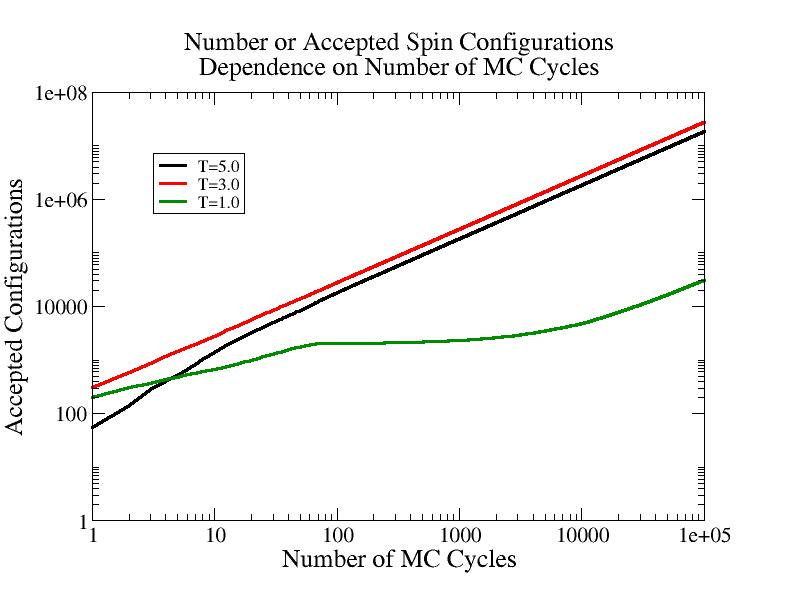
\includegraphics[width=1.1 \textwidth]{acceptplot.jpg}
    \caption{The number of accepted configurations as a function of the number of Monte Carlo Cycles at t=1,3, and 5.l}
\end{figure}

The plot is in log-log scale, indicating a strong linear behavior, with the slope increasing with temperature.  This makes sense because as the temperature increases, more possible configurations are open to the system, allowing for a higher acceptance rate.  As T increase, we expect the slope to approach the total number of configurations.

\subsection{Probability Distributions}

We can also examine the energy probability distribution created by our calculation.  To do this, we performed the same 20 by 20 calculation at T=1 and T=2.4.  Once the system has reached equilibrium, we can histogram the number of times a particular energy is produced by the Monte Carlo cycle.  To ensure that equilibrium was reached, and to make the amount of date tractable, the following plots show the energy results for every 10th calculation between 200,000 and 1,000,000 Monte Carlo cycles.  These plots are shown in Figures \ref{fig:pe1} and \ref{fig:pe2} for T=1.0 and T=2.4, respectively.

To make the comparison between the two cases transparent, the x axis of both plots cover the same energy difference (0.01) and there are 1000 energy bins in each histogram.  It is clear that the P(E) for the T=1.0 case is much sharper and narrower.  This makes sense because, well below the critical temperature, the spins are going to prefer a low energy, aligned spin configuration.

For T=2.4, the distribution becomes much wider.  This is because at higher temperatures, more states become energetically accessible.  This effect can be understood in terms of the energy variance, which is proportional to the heat capacity.  The heat capacities for T=1 and T=2.4 are about 0.023 and 1.41, respectively.  This means the heat capacity for the T=2.4 case is about 60 times greater than for the T=1 case.  If we take a close look at the P(E)s and zoom in the on energy axis, we can see that the T=2.4 case is about 50 times wider than its T=1 counterpart.  This is consistent with the picture of higher temperature leading to a wider energy distribution and larger energy variance. 

\begin{figure}[H]\label{fig:pe1}
  \centering
    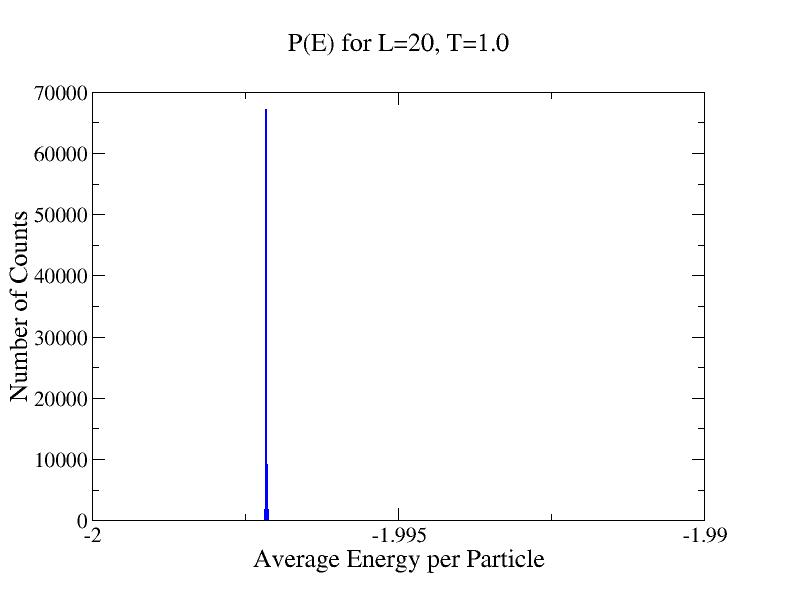
\includegraphics[width=1.1 \textwidth]{pe1.jpg}
    \caption{P(E) for the 20 by 20 lattice with T=1.0}
\end{figure}


\begin{figure}[H]\label{fig:pe2}
  \centering
    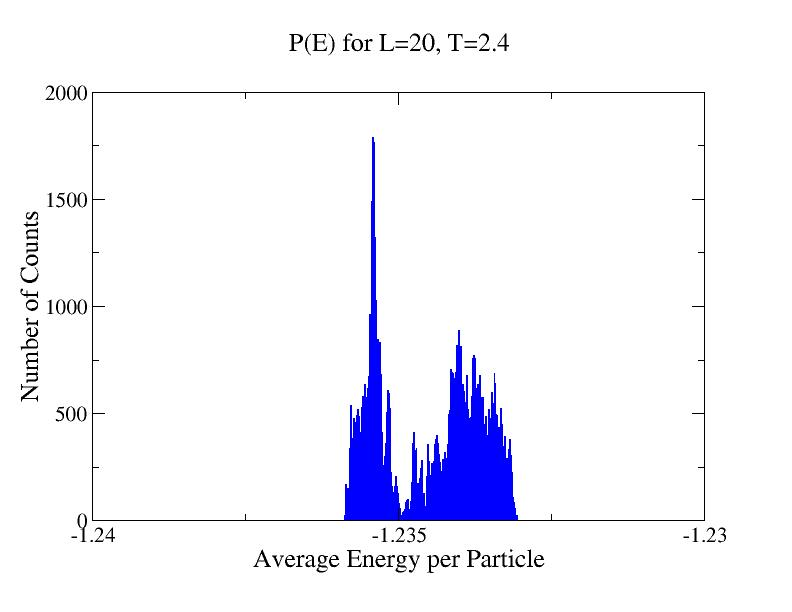
\includegraphics[width=1.1 \textwidth]{p2.jpg}
    \caption{P(E) for the 20 by 20 lattice with T=2.4}
\end{figure}

\section{Conclusions}


\begin{comment}

\begin{figure}[H]\label{fig:compzoom}
  \centering
    \includegraphics[width=1.2\textwidth]{compzoom.eps}
    \caption{A zoomed in view of the convergence to the exact solution}
\end{figure}

\begin{center} 
\begin{tabular}{ |c|c|c|c| }
\hline
Size of Matrix ($10^n$) & General & Tailored & LU \\
\hline
1& 3.00 E -6 & 3.00 E -6 & 2.40 E -5\\ 
2 & 4.00 E -6 & 4.00 E -6 & 1.71 E -3 \\ 
3 & 3.90 E -5 & 1.90 E -5 & 1.93\\ 
4 & 3.79 E -4 & 2.09 E -4 & N/A\\ 
5 & 3.38 E -3 & 1.51 E -3  & N/A\\ 
6 & 2.87 E -2 & 1.53 E -2 & N/A\\ 
7 & 3.16 E -1 & 1.73 E -1& N/A\\ 
\hline
\end{tabular}
\label{table:test}
\end{center}

\end{comment}

\begin{thebibliography}{9}

\bibitem{LectureNotes} 
Hjorth-Jensen, Morten. 
Computational Physics, Lecture Notes Fall 2015. 
August 2015.

\bibitem{Curie}
McGlohon et. al.xm
Curie Temperature, 2012.
https://www.nhn.ou.edu/~johnson/Education/Juniorlab/Magnetism/2013F-CuriePoint.pdf

\bibitem{otherising}
Stauffer, D.
Social Applications of two-dimensional Ising models.
arXiv:0706.3983.

\end{thebibliography}



% ------------------- end of main content ---------------

\end{document}

